% ============================================================
%  PBL Presentation - IMU-Based Tremor Classification
%  FIXED VERSION: text overflow, column balance, font sizes
%  Compiler: pdflatex (run twice) or latexmk -pdf
% ============================================================
\documentclass[aspectratio=169, 11pt]{beamer}

% ── Theme ────────────────────────────────────────────────────
\usetheme{Madrid}
\usecolortheme{whale}
\usefonttheme{professionalfonts}
\setbeamertemplate{navigation symbols}{}
\setbeamertemplate{footline}[frame number]

% ── Packages ─────────────────────────────────────────────────
\usepackage[T1]{fontenc}
\usepackage[utf8]{inputenc}
\usepackage{lmodern}
\usepackage{amsmath, amssymb}
\usepackage{booktabs}
\usepackage{graphicx}
\usepackage{xcolor}
\usepackage{tikz}
\usepackage{pgfplots}
\pgfplotsset{compat=1.18}
\usetikzlibrary{arrows.meta, positioning, shapes.geometric,
                fit, backgrounds, calc}
\usepackage{listings}
\usepackage{multirow}
\usepackage{hyperref}

% ── Custom colours ───────────────────────────────────────────
\definecolor{pblblue}{RGB}{0, 84, 166}
\definecolor{pblorange}{RGB}{220, 100, 30}
\definecolor{pblgreen}{RGB}{30, 140, 80}
\definecolor{pblgray}{RGB}{100, 100, 110}
\definecolor{codebg}{RGB}{245, 245, 248}

\setbeamercolor{structure}{fg=pblblue}
\setbeamercolor{block title}{bg=pblblue, fg=white}
\setbeamercolor{block body}{bg=blue!5}
\setbeamercolor{alertblock title}{bg=pblorange, fg=white}
\setbeamercolor{alertblock body}{bg=orange!8}
\setbeamercolor{exampleblock title}{bg=pblgreen, fg=white}
\setbeamercolor{exampleblock body}{bg=green!6}

% ── Listings style ───────────────────────────────────────────
\lstset{
  backgroundcolor=\color{codebg},
  basicstyle=\ttfamily\tiny,           % FIX: was \scriptsize, too wide
  keywordstyle=\color{pblblue}\bfseries,
  commentstyle=\color{pblgray}\itshape,
  stringstyle=\color{pblorange},
  breaklines=true,
  breakatwhitespace=true,              % FIX: added for better wrapping
  frame=single,
  framerule=0.4pt,
  rulecolor=\color{pblgray!50},
  language=Python,
  showstringspaces=false,
  tabsize=2,
}

% ── Global spacing tweaks ────────────────────────────────────
\setlength{\leftmargini}{1em}         % FIX: tighter list indent
\setlength{\leftmarginii}{0.8em}

% ── Metadata ─────────────────────────────────────────────────
\title[IMU Tremor Classification]{%
  Wrist IMU--Based Tremor Classification\\
  for Parkinson's Disease Screening}
\subtitle{PBL on ECE - Final Presentation}
\author{Ahmed Sameh - 120230134 \\ Faris Essam - 120230124 \\ Mohab Harfoush - 120230112 \vspace{0.5em} \\ {\small Presented to: \\ Dr. Adel Bedair \\ Dr. Asano Tanemasa}   }
\institute{Egypt - Japan University of Science and Technology}
\date{April 29, 2026}

% ============================================================
\begin{document}
% ============================================================

% ── Title slide ──────────────────────────────────────────────
\begin{frame}
  \titlepage
\end{frame}

% ── Outline ──────────────────────────────────────────────────
\begin{frame}{Outline}
  \tableofcontents
\end{frame}

% ============================================================
\section{Problem Definition \& Motivation}
% ============================================================

\begin{frame}{The Clinical Problem}
  \begin{columns}[T]
    \column{0.52\textwidth}
      \begin{alertblock}{Key Facts}
        \small                          % FIX: explicit size to prevent overflow
        \begin{itemize}
          \item Parkinson's Disease (PD) affects \textbf{10 million} people worldwide
          \item Average diagnostic delay: \textbf{4--6 years} after symptom onset
          \item Early detection improves treatment outcomes
          \item Gold-standard diagnosis requires specialist, DaTscan, and longitudinal observation
        \end{itemize}
      \end{alertblock}
      \vspace{0.3em}
      \begin{block}{Motivation}
        \small
        A low-cost wearable screening device could flag at-risk patients
        \emph{before} clinical deterioration, routing them to specialists earlier.
      \end{block}
    \column{0.45\textwidth}           % FIX: widened slightly to give chart room
    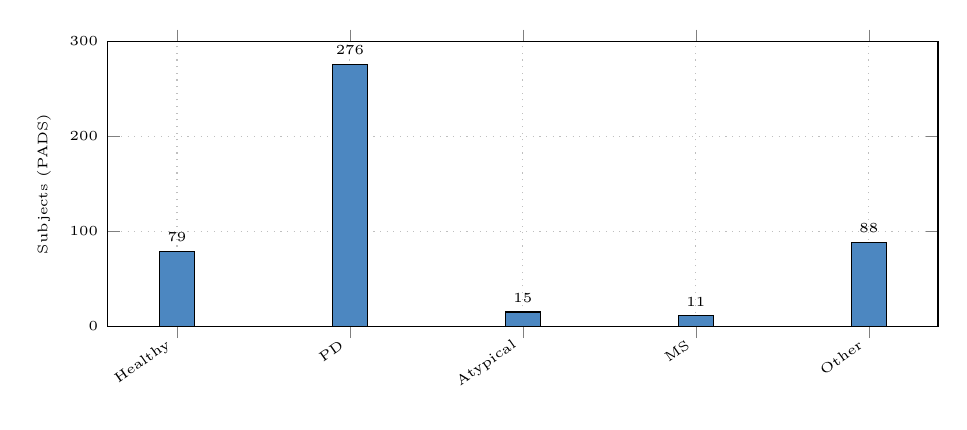
\begin{tikzpicture}
        \begin{axis}[
          width=\textwidth, height=5.2cm,
          ybar, bar width=0.45cm,
          symbolic x coords={Healthy, PD, Atypical, MS, Other},
          xtick=data,
          xticklabel style={rotate=35, anchor=east, font=\tiny},
          ylabel={Subjects (PADS)},
          ylabel style={font=\tiny},
          ymin=0, ymax=300,
          nodes near coords,
          nodes near coords style={font=\tiny},
          tick label style={font=\tiny},
          grid=major, grid style={dotted},
        ]
          \addplot[fill=pblblue!70] coordinates {
            (Healthy, 79) (PD, 276) (Atypical, 15)
            (MS, 11) (Other, 88)};
        \end{axis}
      \end{tikzpicture}
      \vspace{0.1em}
      {\tiny PADS Dataset - 469 subjects, 5 classes}
  \end{columns}
\end{frame}

% ------------------------------------------------------------
\begin{frame}{Why Is This Hard?}
  \begin{exampleblock}{The Core Challenge}
    \small
    All tremor conditions oscillate in the \textbf{same 4--6 Hz band}.
    Frequency alone does not separate them - and treating all motor
    tasks as interchangeable makes the problem worse.
  \end{exampleblock}

  \vspace{0.4em}
  \begin{columns}[T]
    \column{0.48\textwidth}
      \small
      \textbf{Why task segregation is required:}
      \begin{itemize}
        \item Resting vs.\ postural difference requires \emph{distinct clinical tasks}
        \item Task-specific signal structure: resting tremor
              $\neq$ postural tremor $\neq$ action tremor
        \item Standard single-stream models struggle to separate
              these varying physiological signals
        \item Bilateral asymmetry \textrightarrow{} needs 2 wrists
      \end{itemize}
    \column{0.48\textwidth}
      \begin{alertblock}{Modeling Complexity}
        \small
        Tremor pathologies are highly varied. 
        Traditional global metrics obscure the exact localized 
        oscillatory patterns needed to securely distinguish 
        Parkinson's from Essential Tremor or other conditions.
      \end{alertblock}
  \end{columns}
\end{frame}

% ============================================================
\section{Solution \& System Overview}
% ============================================================

\begin{frame}{Our Approach: Task-Guided Ensemble}
  \vspace{-0.3em}
  \begin{center}
  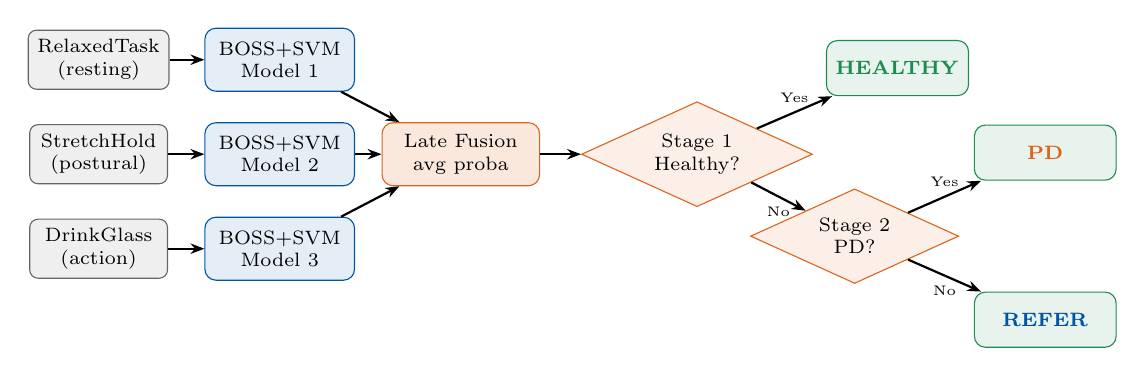
\begin{tikzpicture}[
    node distance=0.5cm and 0.9cm,
    box/.style={draw=pblblue, rounded corners=4pt,
                fill=pblblue!10, minimum width=1.9cm,
                minimum height=0.8cm, align=center,
                font=\scriptsize},
    taskbox/.style={draw=pblgray, rounded corners=3pt,
                fill=pblgray!10, minimum width=1.75cm,
                minimum height=0.75cm, align=center,
                font=\scriptsize},
    dec/.style={draw=pblorange, diamond, aspect=2.2,
                fill=pblorange!10, align=center,
                font=\scriptsize},
    res/.style={draw=pblgreen, rounded corners=4pt,
                fill=pblgreen!10, minimum width=1.8cm,
                minimum height=0.7cm, align=center,
                font=\scriptsize},
    arr/.style={-{Stealth[length=5pt]}, thick},
  ]
    % Three task inputs
    \node[taskbox] (t1) at (0, 1.2)  {RelaxedTask\\(resting)};
    \node[taskbox] (t2) at (0, 0)    {StretchHold\\(postural)};
    \node[taskbox] (t3) at (0,-1.2)  {DrinkGlass\\(action)};

    % Three task-specific BOSS+SVM models
    \node[box] (m1) at (2.3, 1.2)  {BOSS+SVM\\Model 1};
    \node[box] (m2) at (2.3, 0)    {BOSS+SVM\\Model 2};
    \node[box] (m3) at (2.3,-1.2)  {BOSS+SVM\\Model 3};

    % Late fusion
    \node[box, minimum width=2.0cm, fill=pblorange!15,
          draw=pblorange] (fuse) at (4.6, 0) {Late Fusion\\avg proba};

    % Two-stage cascade
    \node[dec] (s1) at (7.6, 0) {Stage 1\\Healthy?};
    \node[res, above right=0.4cm and 0.9cm of s1] (h)
      {\textcolor{pblgreen}{\textbf{HEALTHY}}};
    \node[dec, below right=0.4cm and 0.6cm of s1] (s2) {Stage 2\\PD?};
    \node[res, above right=0.4cm and 0.85cm of s2] (pd)
      {\textcolor{pblorange}{\textbf{PD}}};
    \node[res, below right=0.4cm and 0.85cm of s2] (ref)
      {\textcolor{pblblue}{\textbf{REFER}}};

    \draw[arr] (t1) -- (m1);
    \draw[arr] (t2) -- (m2);
    \draw[arr] (t3) -- (m3);
    \draw[arr] (m1) -- (fuse);
    \draw[arr] (m2) -- (fuse);
    \draw[arr] (m3) -- (fuse);
    \draw[arr] (fuse) -- (s1);
    \draw[arr] (s1) -- node[above, font=\tiny]{Yes} (h);
    \draw[arr] (s1) -- node[below, font=\tiny]{No} (s2);
    \draw[arr] (s2) -- node[above, font=\tiny]{Yes} (pd);
    \draw[arr] (s2) -- node[below, font=\tiny]{No} (ref);
  \end{tikzpicture}
  \end{center}

  \vspace{0.2em}
  \begin{columns}[T]
    \column{0.48\textwidth}
      \begin{block}{Task-Specific Architecture}
        \small We utilize \textbf{three task-specific
        models}, each trained and tuned independently
        for its respective motor task.
      \end{block}
    \column{0.48\textwidth}
      \begin{block}{Late Fusion}
        \small \texttt{predict\_with\_probs} outputs are averaged across tasks
        before the cascade - no feature-level merging.
      \end{block}
  \end{columns}
\end{frame}

% ============================================================
\section{Task-Specific Model Training}
% ============================================================

\begin{frame}{Task-Specific BOSS Models}
  \begin{columns}[T]
    \column{0.50\textwidth}
      \footnotesize
      \textbf{Why task-specific?}
      \begin{itemize}
        \item Motor tasks produce qualitatively different signals
        \item Resting, postural, and action tremors have distinct spectral and temporal structures
        \item Specialized models prevent contradictory patterns from degrading learning
      \end{itemize}
      \vspace{0.2em}
      \textbf{Window size rationale:}
      \begin{itemize}
        \item \texttt{RelaxedTask}: smaller $w$ for high-frequency resting tremor
        \item \texttt{DrinkGlass}: larger $w$ for slow purposive movement
        \item \texttt{StretchHold}: intermediate $w$
      \end{itemize}
    \column{0.47\textwidth}
      \footnotesize
      \textbf{Training procedure:}
      \begin{enumerate}
        \item Collect raw data instances strictly for the targeted clinical task
        \item Define task-specific parameter bounds for $(l, \alpha, w)$
        \item Train MultiBOSS ensemble over the delimited hyperparameter grid
        \item Fit StandardScaler + downstream SVM classifier
        \item Persist the isolated, task-optimized model pipeline
      \end{enumerate}
  \end{columns}
\end{frame}

% ------------------------------------------------------------
\begin{frame}{Late Fusion: Combining Task Predictions}
  \begin{exampleblock}{Why late fusion over feature fusion?}
    \small
    Averaging \texttt{predict\_with\_probs} outputs keeps each task model
    fully independent. Feature concatenation would couple the
    hyperparameter spaces and require joint retraining whenever
    one task model changes.
  \end{exampleblock}

  \vspace{0.4em}
  \begin{columns}[T]
    \column{0.52\textwidth}
      \small
      \textbf{Fusion procedure per subject:}
      \begin{enumerate}
        \item Retrieve \texttt{.npy} files for each of the 3 tasks
        \item Run each file through its task-specific BOSS+SVM
              pipeline $\rightarrow$ probability vector $\mathbf{p}_k$
        \item Average: $\bar{\mathbf{p}} = \frac{1}{K}\sum_{k=1}^{K}\mathbf{p}_k$
        \item Feed $\bar{\mathbf{p}}$ into Stage 1 cascade decision
        \item \textbf{Fallback:} if a subject is missing a task,
              average over remaining tasks only
      \end{enumerate}
    \column{0.45\textwidth}
      \small
      \textbf{Evaluation:}
      \begin{itemize}
        \item \texttt{StratifiedKFold} grouped by \texttt{subject\_id}
        \item Prevents any subject's windows appearing in both
              train and test
        \item Final metrics: macro F1, balanced accuracy,
              per-class precision / recall
        \item Robust assessment across 5 diagnostic classes
      \end{itemize}
  \end{columns}
\end{frame}

% ------------------------------------------------------------
\begin{frame}{Live Inference State-Machine Protocol}
  \small
  \textbf{From stateless inference to a structured clinical session:}

  \vspace{0.4em}
  \begin{center}
  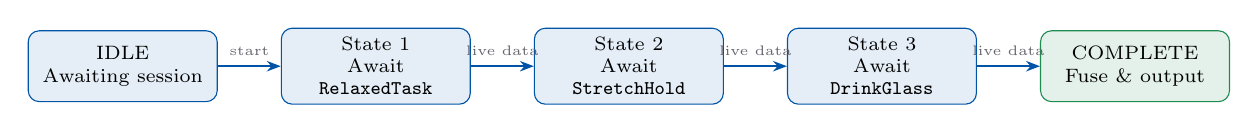
\begin{tikzpicture}[
    node distance=0.4cm and 0.8cm,
    st/.style={draw=pblblue, rounded corners=4pt, fill=pblblue!10,
               minimum width=2.4cm, minimum height=0.9cm,
               align=center, font=\scriptsize},
    arr/.style={-{Stealth[length=5pt]}, thick, pblblue},
    lab/.style={font=\tiny, pblgray},
  ]
    \node[st] (s0) {IDLE\\Awaiting session};
    \node[st, right=of s0] (s1) {State 1\\Await\\ \texttt{RelaxedTask}};
    \node[st, right=of s1] (s2) {State 2\\Await\\ \texttt{StretchHold}};
    \node[st, right=of s2] (s3) {State 3\\Await\\ \texttt{DrinkGlass}};
    \node[st, right= of s3, fill=pblgreen!12, draw=pblgreen] (done)
      {COMPLETE\\Fuse \& output};

    \draw[arr] (s0) -- node[above, lab]{start} (s1);
    \draw[arr] (s1) -- node[above, lab]{live data} (s2);
    \draw[arr] (s2) -- node[above, lab]{live data} (s3);
    \draw[arr] (s3) -- node[above, lab]{live data} (done);
  \end{tikzpicture}
  \end{center}

  \vspace{0.3em}
  \begin{columns}[T]
    \column{0.50\textwidth}
      \textbf{Real-Time Controller:}
      \begin{itemize}
        \item Ingests live data stream from the ESP32 hardware
        \item Loads all task-specific models into RAM at startup
        \item Maintains continuous per-session state 
        \item Emits final ensemble diagnosis immediately after State 3
      \end{itemize}
    \column{0.47\textwidth}
      \textbf{Hardware Integration:}
      \begin{itemize}
        \item ESP32 buffer directly triggers model inference pipeline
        \item Completely seamless transition from physical movement to prediction vector
        \item Robust error handling for truncated or interrupted signal windows
      \end{itemize}
  \end{columns}
\end{frame}

% ============================================================
\section{Hardware Implementation}
% ============================================================

\begin{frame}{Hardware Setup}
  \begin{columns}[T]
    \column{0.50\textwidth}
      \small
      \textbf{Components:}
      \begin{itemize}
        \item ESP32 microcontroller
        \item MPU-6050 IMU (accel + gyro)
        \item Sampling rate: \textbf{100 Hz}
        \item Window: \textbf{1024 samples} (10 seconds)
        \item USB serial / BLE to host
      \end{itemize}
      \vspace{0.2em}
      \textbf{Data flow (per task):}
      \begin{enumerate}
        \item IMU $\xrightarrow{\text{I}^2\text{C}}$ ESP32 buffer
        \item Buffer fills ($1024 \times 6$ samples)
        \item Send over serial as .npy file
        \item Host ingests live stream and decodes
        \item State machine invokes rapid
              task-specific model inference
      \end{enumerate}
    \column{0.477\textwidth}
      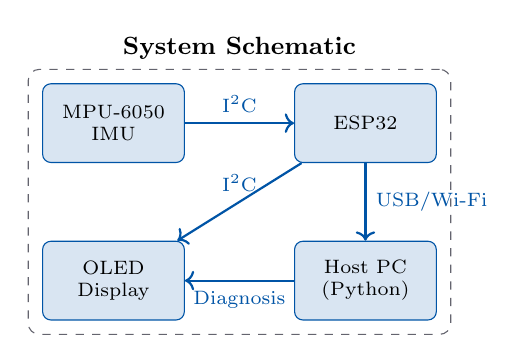
\begin{tikzpicture}[font=\scriptsize,
        ic/.style={draw=pblblue, fill=pblblue!15,
                   minimum width=1.8cm, minimum height=1.0cm,
                   rounded corners=3pt, align=center},
        wire/.style={thick, pblblue},
      ]
        \node[ic] (mpu) at (0,0) {MPU-6050\\IMU};
        \node[ic] (esp) at (3.2,0) {ESP32};
        \node[ic] (host) at (3.2,-2.0) {Host PC\\(Python)};
        \node[ic] (oled) at (0,-2.0) {OLED\\Display};

        \draw[wire, ->] (mpu) -- node[above]{I\textsuperscript{2}C} (esp);
        \draw[wire, ->] (esp) -- node[right]{USB/Wi-Fi} (host);
        \draw[wire, ->] (host) -- node[below]{Diagnosis} (oled);
        \draw[wire, ->] (esp) -- node[above]{I\textsuperscript{2}C}(oled);

        \node[draw=pblgray, dashed, rounded corners,
              fit=(mpu)(esp)(host)(oled),
              inner sep=5pt,
              label=above:{\small\textbf{System Schematic}}] {};
      \end{tikzpicture}
    \end{columns}
\end{frame}

% ------------------------------------------------------------
\begin{frame}{Data Shapes \& Pipeline}
  \begin{block}{Per-Task Frame}
    \small
    Each task produces one 10-second window:
    \[
      \underbrace{1024}_{\text{time steps}} \times
      \underbrace{6}_{\text{channels}} = 6{,}144 \text{ float32 values}
      \quad \xrightarrow{\text{save}} \texttt{\{task\}.npy}
    \]
    Channels: \texttt{aX, aY, aZ, gX, gY, gZ}
  \end{block}

  \vspace{0.3em}
  \begin{columns}[T]
    \column{0.50\textwidth}
      \small
      \textbf{Per-task processing:}
      \begin{enumerate}
        \item Reshape to $(6, 1024)$
        \item DC removal + bandpass (0.5--20 Hz)
        \item Task-specific BOSS $\rightarrow$ feature vector
        \item Task-specific SVM $\rightarrow$ \texttt{predict\_with\_probs}
        \item State machine stores $\mathbf{p}_k$
      \end{enumerate}
    \column{0.47\textwidth}
      \small
      \textbf{Shape summary:}\\[0.3em]
      \begin{tabular}{ll}
        \toprule
        Stage & Shape \\
        \midrule
        Raw window & $(6, 1024)$ \\
        After BOSS & $(1, d),\ d \leq 42$ \\
        Per-task prob & $(1, C)$ \\
        Fused prob & $(1, C)$ \\
        \bottomrule
      \end{tabular}\\[0.3em]
      {\footnotesize $C$ = number of classes; fusion averages
      $K \leq 3$ probability vectors}
  \end{columns}
\end{frame}

% ============================================================
\section{Model Pipeline}
% ============================================================

\begin{frame}{Why Dictionary-Based Classification?}
  \begin{exampleblock}{Motivation}
    \small
    Tremor is not defined by a single frequency peak but by
    \textbf{repeating symbolic patterns}. Dictionary methods capture this naturally.
  \end{exampleblock}

  \vspace{0.4em}
  \begin{columns}[T]
    \column{0.48\textwidth}
      \small
      \textbf{FFT / band-power (traditional approach):}
      \begin{itemize}
        \item Summarises global frequency content
        \item Loses temporal ordering
        \item All tremor types share 4--6 Hz band
        \item Poor inter-class separability (confirmed by STFT)
      \end{itemize}
    \column{0.48\textwidth}
      \small
      \textbf{Dictionary / symbolic approach:}
      \begin{itemize}
        \item Captures \emph{which patterns occur} and \emph{how often}
        \item Encodes local shape, not just frequency
        \item Robust to amplitude variation across patients
        \item Works on raw or lightly pre-processed signal
      \end{itemize}
  \end{columns}

  \vspace{0.4em}
  \begin{alertblock}{Key Insight}
    \small
    PD tremor is \textbf{rhythmically regular}: the same short subsequence
    repeats. BOSS counts exactly these repetitions.
  \end{alertblock}
\end{frame}

% ------------------------------------------------------------
\begin{frame}{SFA: Symbolic Fourier Approximation}
  \small                                % FIX: set frame-level size
  \textbf{Step 1 - Dimensionality Reduction via DFT:}
  \[
    \hat{x}_1, \hat{x}_2, \ldots, \hat{x}_l = \mathrm{DFT}(x)[1{:}l],
    \quad l \ll T
  \]
  Keep only the first $l$ Fourier coefficients of each subsequence.

  \vspace{0.4em}
  \textbf{Step 2 - Quantisation (MCB):}
  \begin{itemize}
    \item Fit breakpoints on training data distribution (per coefficient)
    \item Map each coefficient to one of $\alpha$ symbols $\in \{a, b, c, \ldots\}$
    \item Each subsequence becomes a \textbf{word} of length $l$
  \end{itemize}

  \vspace{0.3em}
  \begin{center}
  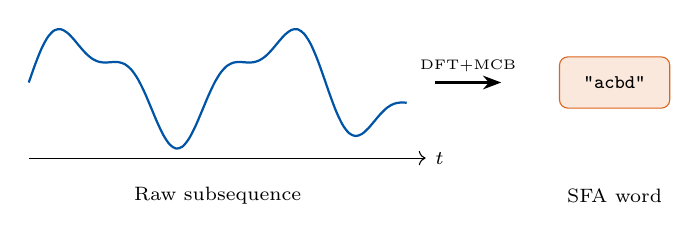
\begin{tikzpicture}[font=\scriptsize, scale=1.2]  % FIX: scaled down
    \draw[pblblue, thick] plot[smooth, domain=0:4, samples=60]
      (\x, {0.5*sin(3*\x r) + 0.2*sin(7*\x r)});
    \draw[->] (0,-0.8) -- (4.2,-0.8) node[right]{$t$};
    \node at (2,-1.2) {Raw subsequence};

    \draw[-{Stealth}, thick] (4.3,0) -- (5.0,0)
      node[midway, above]{\tiny DFT+MCB};

    \node[draw=pblorange, fill=pblorange!15,
          minimum width=1.4cm, minimum height=0.65cm,
          rounded corners=3pt] at (6.2,0) {\texttt{"acbd"}};
    \node at (6.2,-1.2) {SFA word};
  \end{tikzpicture}
  \end{center}
\end{frame}

% ------------------------------------------------------------
\begin{frame}{BOSS: Bag-of-SFA-Symbols}
  \small
  \textbf{Step 3 - Build histogram over a full window:}
  \begin{enumerate}
    \item Slide a window of length $w$ (step 1) across the time series
    \item Convert each position to an SFA word
    \item \textbf{Numerosity reduction}: keep only the first occurrence
          of consecutive identical words
    \item Count occurrences $\rightarrow$ \textbf{word histogram} = feature vector
  \end{enumerate}

  \vspace{0.2em}
  \begin{center}
  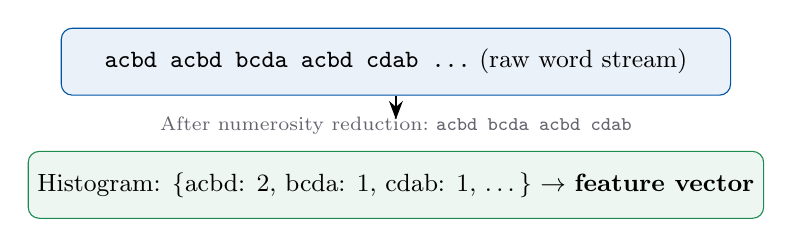
\begin{tikzpicture}[font=\scriptsize]
    \node[draw=pblblue, fill=pblblue!8, rounded corners,
          minimum width=8.5cm, minimum height=0.85cm] (sig)
      {\small \texttt{acbd acbd bcda acbd cdab \ldots}\ (raw word stream)};
    \node[below=0.15cm of sig, pblgray]
      {After numerosity reduction:\ \texttt{acbd\ bcda\ acbd\ cdab}};
    \node[draw=pblgreen, fill=pblgreen!8, rounded corners,
          minimum width=8.5cm, minimum height=0.85cm,
          below=0.7cm of sig]
      {\small Histogram: \{acbd: 2,\ bcda: 1,\ cdab: 1,\ \ldots\} $\rightarrow$ \textbf{feature vector}};
    \draw[-{Stealth}, thick] (sig.south) -- ++(0,-0.3);
  \end{tikzpicture}
  \end{center}

  \vspace{0.2em}
  \begin{block}{Complexity}
    \small
    Training: $\mathcal{O}(n \cdot T)$ \quad
    Prediction: $\mathcal{O}(T)$ - fast enough for embedded deployment.
  \end{block}
\end{frame}

% ------------------------------------------------------------
\begin{frame}{MultiBOSS: Ensemble over Hyperparameters}
  \small
  \textbf{Problem:} BOSS has three hyperparameters - word length $l$,
  alphabet size $\alpha$, subsequence length $w$.
  No single setting is optimal for all patterns.

  \vspace{0.4em}
  \textbf{Solution - MultiBOSS:}
  \begin{enumerate}
    \item Train BOSS classifiers for a \emph{grid} of $(l, \alpha, w)$ combinations
    \item Extract words across multiple timescales without discarding parallel models
    \item \textbf{Concatenate} all extracted histograms into one master feature vector:
      \[
        \mathbf{f} = \bigl[\,\mathrm{hist}_{(l_1,\alpha_1,w_1)} \;\|\;
                              \mathrm{hist}_{(l_2,\alpha_2,w_2)} \;\|\;
                              \cdots \,\bigr]
      \]
    \item Feed the concatenated vector to a single downstream classifier
  \end{enumerate}

  \vspace{0.3em}
  \begin{exampleblock}{Why this matters for tremor}
    \small
    Tremor patterns exist at multiple timescales simultaneously.
    A short window captures oscillation shape; a long window captures rhythmic
    regularity. MultiBOSS learns both simultaneously.
  \end{exampleblock}
\end{frame}

% ------------------------------------------------------------
\begin{frame}{SVM Classifier with StandardScaler Pipeline}
  \begin{block}{sklearn Pipeline}
    \small\ttfamily
    Pipeline([("scaler", StandardScaler()),\\
    \hspace{2.2em}("svm", SVC(kernel="rbf", class\_weight="balanced"))])
  \end{block}  % FIX: split long line to avoid horizontal overflow

  \vspace{0.4em}
  \begin{columns}[T]
    \column{0.48\textwidth}
      \small
      \textbf{Why StandardScaler?}
      \begin{itemize}
        \item BOSS histograms have variable scales\\
          (common words: count $\gg 100$; rare: count $= 0$)
        \item RBF kernel uses Euclidean distance -
          unscaled features dominate
        \item $z = (x - \mu)/\sigma$, fitted on train only
      \end{itemize}
    \column{0.48\textwidth}
      \small
      \textbf{Why SVM + RBF?}
      \begin{itemize}
        \item BOSS histograms are sparse, high-dimensional
        \item RBF handles non-linear boundaries implicitly
        \item \texttt{class\_weight="balanced"} corrects
          21:1 class imbalance without oversampling
      \end{itemize}
  \end{columns}

  \vspace{0.3em}
  \begin{alertblock}{No Data Leakage}
    \small
    Scaler is inside the Pipeline - \texttt{fit} is called only on
    training data; val/test use \texttt{transform} only.
  \end{alertblock}
\end{frame}

% ============================================================
\section{Model Evaluation}
% ============================================================

\begin{frame}{Evaluation Strategy}
  \begin{columns}[T]
    \column{0.50\textwidth}
      \small
      \textbf{Group-level subject split:}
      \begin{itemize}
        \item 469 subjects, \texttt{StratifiedKFold} grouped
              by \texttt{subject\_id}
        \item All windows from one subject stay in the same fold
        \item Prevents patient leakage across splits
        \item Subjects missing a task: averaged over remaining
              tasks (not dropped)
      \end{itemize}
      \vspace{0.3em}
      \textbf{Metrics:}
      \begin{itemize}
        \item Macro F1 (primary)
        \item Balanced accuracy
        \item Per-class precision, recall, F1
        \item Cascaded end-to-end recall
      \end{itemize}
    \column{0.48\textwidth}
      \small
      \textbf{Why not raw accuracy?}
      \begin{itemize}
        \item Class ratio: 3312 PD vs.\ 180 Other
        \item Predicting PD always $\Rightarrow$ 73\% accuracy
        \item Macro F1 penalises ignoring minority classes
      \end{itemize}
      \vspace{0.3em}
      \textbf{Ensemble evaluation:}
      \begin{itemize}
        \item Patient-level majority vote is applied
              within each task window set
        \item Late fusion happens \emph{after} patient-level
              vote per task
        \item Follows the logical clinical workflow
      \end{itemize}
  \end{columns}
\end{frame}

% ------------------------------------------------------------
\begin{frame}{Results}
  \begin{columns}[T]
    \column{0.50\textwidth}
      \begin{block}{Stage 1: Healthy vs.\ Tremor}
        \footnotesize
        \begin{tabular}{lcc}
          \toprule
          Class & Prec. & Recall \\
          \midrule
          Healthy & 0.40 & 0.42 \\
          Tremor  & 0.88 & 0.87 \\
          \midrule
          \textbf{Macro F1} & \multicolumn{2}{c}{\textbf{0.643}} \\
          \textbf{Bal.\ Acc.} & \multicolumn{2}{c}{\textbf{0.647}} \\
          \bottomrule
        \end{tabular}
      \end{block}
      \vspace{0.1em}
      \begin{block}{Stage 2: PD vs.\ Other Tremor}
        \footnotesize
        \begin{tabular}{lcc}
          \toprule
          Class & Prec. & Recall \\
          \midrule
          Other Tremor & 0.39 & 0.32 \\
          Parkinson's  & 0.74 & 0.79 \\
          \midrule
          \textbf{Macro F1} & \multicolumn{2}{c}{\textbf{0.559}} \\
          \textbf{Bal.\ Acc.} & \multicolumn{2}{c}{\textbf{0.558}} \\
          \bottomrule
        \end{tabular}
      \end{block}
    \column{0.48\textwidth}
      \begin{alertblock}{End-to-End Cascaded Recall}
        \footnotesize
        \begin{tabular}{lc}
          \toprule
          Class & Detection Rate \\
          \midrule
          Healthy & 0.42 \\
          Parkinson's & $0.87 \times 0.79 = \mathbf{0.69}$ \\
          Other Tremor & $0.87 \times 0.32 = 0.28$ \\
          \midrule
          Macro Recall & \textbf{0.46} \\
          \bottomrule
        \end{tabular}
      \end{alertblock}
      \vspace{0.1em}
      \begin{exampleblock}{Validation}
        \footnotesize
        The ensemble model flags 87\% of tremor patients for screening
        and isolates 69\% of Parkinsonian tremors.
      \end{exampleblock}
    \end{columns}
\end{frame}

% ------------------------------------------------------------
\begin{frame}{Limitations \& Future Expansion}
  \begin{columns}[T]
    \column{0.48\textwidth}
      \small
      \textbf{Current Scope Constraints:}
      \begin{itemize}
        \item Single wrist classification limits structural tracking of bilateral asymmetry
        \item "Other Tremor" is a heterogeneous class combining 3 underlying conditions
      \end{itemize}
      \vspace{0.4em}
      \textbf{Clinical Scaling:}
      \begin{itemize}
        \item Validate cohort far beyond initial 469 parameters for definitive medical regulations
      \end{itemize}
    \column{0.48\textwidth}
      \small
      \textbf{Next Technical Steps:}
      \begin{itemize}
        \item Two-wrist network enabling synced bilateral cross-referencing
        \item Expand from 3 tasks to a comprehensive motor exam array
        \item Integrate Questionnaire data (NMS score) via stacking
        \item Full on-device standalone TFLite inference directly on ESP32-S3
        \item Longitudinal data extraction for continuous tracking
      \end{itemize}
  \end{columns}

  \vspace{0.5em}
  \begin{block}{Screening vs. Diagnosis}
    \small
    This device is a \textbf{screening tool}. It simply answers: 
    \emph{``Should this person see a neurologist?''}
  \end{block}
\end{frame}

% ============================================================
\section{Conclusion}
% ============================================================

\begin{frame}{Conclusion}
  \small
  \begin{enumerate}
    \item Built \textbf{three task-specific BOSS+SVM models}
          (\texttt{RelaxedTask}, \texttt{StretchHold}, \texttt{DrinkGlass}),
          each with independently tuned MultiBOSS window sizes
    \vspace{0.3em}
    \item Implemented \textbf{late fusion} averaging
          \texttt{predict\_with\_probs} outputs across tasks before the
          two-stage cascade decision
    \vspace{0.3em}
    \item Replaced stateless single-shot inference with a
          \textbf{sequential real-time state-machine protocol}, directly
          enabling seamless hardware integration and continuous evaluation.
    \vspace{0.3em}
    \item Established evaluation under grouped \texttt{StratifiedKFold}
          with explicit missing-task fallback strategy
  \end{enumerate}

  \vspace{0.5em}
  \begin{center}
    \large\textbf{Thank you. Questions?}
  \end{center}
\end{frame}

% ── References ───────────────────────────────────────────────
\begin{frame}{References}
  \small
  \begin{thebibliography}{9}
    \bibitem{pads}
      Klucken et al.\ (2023).
      \textit{PADS: Parkinson's Disease Smartwatch Dataset}.
      PhysioNet. \texttt{doi:10.13026/xxx}

    \bibitem{boss}
      Sch\"{a}fer, P.\ (2015).
      \textit{The BOSS is concerned with time series classification in the
      presence of noise}.
      Data Mining and Knowledge Discovery, 29(6), 1505--1530.

    \bibitem{sktime}
      L\"{o}ning et al.\ (2019).
      \textit{sktime: A unified interface for machine learning with time series}.
      NeurIPS Workshop.

    \bibitem{xceptiontime}
      Rahimian et al.\ (2022).
      \textit{XceptionTime: Independent Time-Step Factorization for Deep
      Time Series Classification}.
      arXiv:2011.11956.
  \end{thebibliography}
\end{frame}

\end{document}
